\chapter{Implementacja}

Problem układania planu zajęć można próbować rozwiązać za pomocą algorytmu \textit{Tabu search}. Jednak podczas implementacji napotkać można dużą ilość przeszkód, związaną ze złożonością problemu układania planu zajęć. Rozmiar generowanego sąsiedztwa czy poziom skomplikowania funkcji oceny to tylko niektóre z nich. Poniżej omówiona została próba implementacji algorytmu oraz specyfikacja wewnętrzna i zewnętrzna powstałej aplikacji.

\section{Implementacja algorytmu}

Implementacja algorytmu napisana jest w języku C\#. Język ten został wybrany, z uwagi na dużą liczbę darmowych bibliotek oraz dostępu do bardzo dobrej dokumentacji technicznej. Nie bez znaczenia pozostał też fakt dużej popularności języka, co przekłada się na większą możliwość uzyskania pomocy na forach programistycznych. Szczegółowy opis języka znajduje się w podrozdziale o specyfikacji wewnętrznej.

\subsection{Wczytywanie danych}

Pierwszym problemem, który stanął przed autorem tej pracy, było wczytywanie danych z formatu XHSTT. Format ten został szczegółowo omówiony w poprzednim rozdziale. Dane zostały zapisane w języku XML. Skorzystano więc z biblioteki systemowej  \textit{Xml.Linq}, która pozwala traktować dokument XML jako bazę danych i wysyłać do niego stosowne zapytania. Przykład wczytywania instancji za pomocą tej biblioteki przedstawiony został na rysunku 5.1. Biblioteka \textit{Xml.Linq} stanowiła spore ułatwienie, jednak w dalszym ciągu problemem pozostał złożony charakter dokumentu, ponieważ każde zagnieżdżenie musiało być wczytane za pomocą odpowiedniej linii kodu. 

\begin{figure}
	\centering
	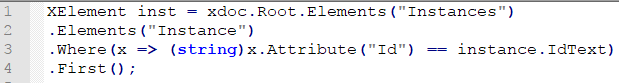
\includegraphics {linqprzyklad}
	\caption{Przykład wczytywania instancji za pomocą biblioteki \textit{Xml.Linq}.}
	\label{fig: linqprzyklad}
\end{figure}

Wczytywane dane zapisywane są w bazie danych, dlatego każde kolejne uruchomienie aplikacji umożliwia pracę na już wczytanych danych.

Jak zostało powiedziane w poprzednich rozdziałach, założono, że wczytane dane zawierają zdarzenia z przypisanymi wcześniej zasobami takimi jak nauczyciel, sala i grupa. Dalsza implementacja algorytmu opiera się na tym założeniu.

\subsection{Generowanie rozwiązania początkowego}

Algorytm \textit{Tabu search} poszukiwanie najlepszego rozwiązania musi rozpocząć od jakiegoś miejsca. Miejscem to nazywane jest rozwiązaniem początkowym. Warto przypomnieć, że algorytm \textit{Tabu search} jest algorytmem heurystycznym. W zależności od tego, w jakim miejscu rozpocznie on poszukiwanie, może uzyskać różne rezultaty po określonej liczbie iteracji. Stworzenie początkowego planu zajęć, gdzie wszystkie zajęcia rozpoczynałyby się w poniedziałek, w pierwszym dostępnym oknie czasowym, mogłoby spowodować znaczne wydłużenie czasu, w którym algorytm znajdzie optymalne rozwiązanie. Wydłużony czas, spowodowany był by bardzo złą oceną takiego planu i dłuższą drogą, jaką algorytm musi pokonać, by dojść do rozwiązania optymalnego. Zdecydowano się więc na wprowadzenie elementu probabilistycznego, by w prosty sposób zróżnicować początkowy plan zajęć. Każdemu wydarzeniu przypisywane jest losowe okno czasowe. Dobrym pomysłem było by zastosowanie prostego algorytmu, który utworzył by początkowy plan zajęć z jeszcze lepszą oceną, jednak, z uwagi na ograniczony czas implementacji, zdecydowano się pozostać przy rozwiązaniu losowym.

\subsection{Generowanie dostępnych ruchów algorytmu}

By swobodniej generować sąsiedztwo niezbędne w dalszym działaniu algorytmu, zdecydowano się na wygenerowanie wszystkich dostępnych ruchów dla jednego kroku algorytmu. Jako dostępny ruch rozumiana jest para: wydarzenie i okno czasowe. Oznacza to, że wybranemu wydarzeniu przyporządkowane jest określone okno czasowe. Generowane są więc wszystkie pary, których liczba równa jest liczbie wydarzeń pomnożonej razy liczbę okien czasowych. Tak zinterpretowany ruch, może być w łatwy sposób wykorzystany przy generacji sąsiedztwa. Co więcej, tak wygenerowane pary nie są zależne od aktualnego rozwiązania i, dla każdego kroku algorytmu, są zawsze takie same (o ile nie znajdują się na liście Tabu). Dzięki temu, można łatwo identyfikować ruch jako parę indeksów i przechowywać go na liście Tabu. Liczba wszystkich dostępnych ruchów określa rozmiar sąsiedztwa, które algorytm powinien przeszukać w jednym kroku. Ponieważ liczba ta jest duża, konieczne było ograniczenie przeszukiwanego sąsiedztwa.

\subsection{Generowanie i ocenianie sąsiedztwa dla wybranego rozwiązania}

W ramach jednej iteracji algorytm powinien wygenerować sąsiedztwo dla wybranego rozwiązania, ocenić każdego sąsiada i wybrać najlepszego z nich. Ponieważ, funkcja oceny rozwiązania jest bardzo kosztowna, konieczne było ograniczenie rozmiaru przeszukiwanego sąsiedztwa. Parametr określający jego rozmiar jest jednym z parametrów wejściowych algorytmu. Po raz kolejny zdecydowano się wprowadzić element probabilistyczny. Z puli dostępnych ruchów wybierane są losowe jednostki. Każdy z wylosowanych ruchów wykonywany jest na aktualnym rozwiązaniu, tworząc nowe rozwiązanie, wchodzące w skład sąsiedztwa rozwiązania aktualnego. Tak wygenerowane sąsiedztwo jest oceniane i wybierane jest rozwiązanie najlepsze spośród dostępnych. Ruch, który doprowadził nas do rozwiązania najlepszego trafia na listę Tabu. Następnie wybrane rozwiązanie porównywane jest z rozwiązaniem globalnie najlepszym, jakie do tej pory udało się znaleźć. Jeżeli nowo wybrane rozwiązanie jest lepsze, staje się wtedy rozwiązaniem najlepszym globalnie. Ostatnim krokiem w ramach jednej iteracji algorytmu jest aktualizowanie listy Tabu. Dla każdego elementu na liście aktualizowany jest czas trwania w Tabu i, jeżeli jest on równy zeru, ruch trafia z powrotem do listy dostępnych ruchów algorytmu.

\subsection{Funkcja oceny rozwiązania}

Najtrudniejszym elementem implementacji była funkcja oceny danego rozwiązania. Z uwagi na konieczność sprawdzania wielu warunków i iteracji po wielu elementach, jest to najbardziej czasochłonna część wykonania algorytmu. Wszystkie ograniczenia, które ma spełniać otrzymany plan zajęć, muszą być zaimplementowane w tej funkcji. Funkcja ta bezpośrednio decyduje o jakości otrzymanego planu i daje duże możliwości, by rozwinąć ją w przyszłości.

Zdecydowano się wybrać do implementacji następujące ograniczenia:
\begin{itemize}
\item przypisanie wszystkim zdarzeniom określonego czasu,
\item unikanie konfliktów między zasobami,
\item unikanie dzielenia zajęć trwających dłużej niż jedno okno czasowe,
\item minimalizacja pustych okien czasowych między zdarzeniami dla grup uczniów.
\end{itemize}

Każde z tych ograniczeń posiada określoną wartość kary, która zostanie dodana do końcowej oceny rozwiązania, za każdym razem, gdy ograniczenie nie zostanie spełnione.

Każde zdarzenie musi mieć przypisane okno czasowe. Podczas oceny tego ograniczenia sprawdzane są wszystkie dostępne wydarzenia. Za każdym razem, gdy któreś z wydarzeń nie będzie miało przypisanego czasu, nałożona zostanie odpowiednia kara. Ograniczenie to miało zastosowanie tylko w początkowej fazie implementacji algorytmu, ponieważ aktualnie, każde zdarzenie, już podczas generacji rozwiązania początkowego ma przypisane okno czasowe. Nie ma również możliwości, by algorytm usunął przypisane okno czasowe. Jedynymi zmianami może być przypisanie nowego okna czasowego.

Unikanie konfliktów między zasobami. Ograniczenie to sprawdzane jest w następujący sposób: dla każdego okna czasowego wyszukiwane są wszystkie zdarzenia, które w nim występują. Konieczne jest również przeszukanie dwóch okien czasowych w tył, by sprawdzić czy nie ma tam zajęć o długości dwóch lub trzech jednostek czasu. Po znalezieniu wszystkich zdarzeń, przeszukiwane są wszystkie zasoby, do nich przypisane. Każdy zasób sprawdzany jest pod kątem wystąpienia po raz kolejny w tym samym oknie czasowym. Za każde dodatkowe występnie zasobu nakładana jest stosowna kara. Sprawdzanie tego ograniczenia ma największą złożoność obliczeniową ponieważ wymaga wielokrotnego sprawdzania zasobów.

Unikanie dzielenia zajęć trwających dłużej niż jedno okno czasowe. To ograniczenie może być złamane na przykład w przypadku, gdy zajęcia o czasie trwania dwóch okien czasowych przypisane są na ostatnie okno czasowe danego dnia. Wtedy druga godzina zajęć przypisana jest w pierwszym oknie czasowym dnia następnego. Nie jest to zjawisko pożądane. By wykryć złamanie tego ograniczenia konieczne jest sprawdzenie wszystkich zajęć o czasie trwania dłuższym niż jeden. Dla każdego z tych zajęć sprawdzane są kolejne okna czasowe występujące po nim (w zależności od długości zajęć jest to jedno lub dwa okna czasowe). Jeżeli okna czasowe przypadające na jedno zajęcie należą do różnych dni, to nakładana jest ustalona kara.

Wszystkie dotychczasowe ograniczenia można było określić jako ograniczenia twarde. Kara za ich złamanie była bardzo wysoka. Ostatnie ograniczenie jest ograniczeniem miękkim. W kara za jego złamanie to około 10\% wartości kary poprzednich ograniczeń. Minimalizacja pustych okien czasowych między zdarzeniami dla grup uczniów nie jest obowiązkowa dla poprawnego planu zajęć. Jest jednak zjawiskiem pożądanym przez uczniów. By sprawdzić te ograniczenie konieczne jest przeszukanie planu dla każdej klasy z osobna. Jeżeli dla danej klasy, w danym dniu, wystąpiły już zajęcia, następnie wystąpiło puste okno czasowe, a po nim kolejne zajęcia to nałożona zostanie kara. Kara jest zależna od liczby pustych okien czasowych między zajęciami.

\section{Specyfikacja wewnętrzna}

Poprzedni podrozdział miał na celu przybliżyć czytelnikowi pomysł i sposób w jaki zaimplementowany został algorytm \textit{Tabu search}. Ten podrozdział zawiera szczegóły techniczne implementacji, opis użytych technologii, używanych klas oraz zawiera najistotniejsze fragmenty kodu.

\subsection{Użyte technologie i narzędzia}

\begin{itemize}
	\item Język programowania C\# - jest to obiektowy język programowania, którego początki sięgają roku 1998. Został zaprojektowany dla firmy Microsoft przez Andersa Hejlsberga. Program napisany w tym języku jest kompilowany do języka \textit{Common Intermediate Language} (CIL), który jest wykonywany w środowisku \textit{.NET Framework}. Jest to język prosty, o dużych możliwościach i wielu cechach wspólnych z językami programowania C++ oraz Java \cite{Csharp}. 
	
	\item Technologia Linq - Language-Integrated Query (LINQ) to technologia zapytań w języku zintegrowanym, pozwalająca odczytywać dane, pochodzące z różnych źródeł, w postaci obiektów. Udostępnia szereg funkcji filtrujących i wyszukujących, które, odpowiednio użyte, w znacznej mierze przyspieszają działanie programu. W implementacji algorytmu, którego dotyczy ta praca, zapytania Linq ułatwiają komunikację z bazą danych oraz czytanie dokumentów XML.
	
	\item Windows Forms - interfejs programowania graficznych aplikacji należący do środowiska \textit{.NET Framework}. Jest to technologia tworzenia aplikacji z graficznym interfejsem użytkownika, umożliwiająca obsługę zdarzeń napływających od użytkownika. Obecnie wypierana przez technologię  \textit{WPF}, mimo to, dzięki swej prostocie i przejrzystości, jest dalej używana przez programistów.
	 
	\item Entity Framework - jest to wolne oprogramowanie typu Object Relational Mapping (ORM), pozwalające odwzorować relacyjną bazę danych za pomocą architektury obiektowej. Dzięki temu narzędziu programista może w łatwy sposób zaprojektować bazę danych nie mając wiedzy na temat języka SQL. Stosując podejście \textit{code first} można zaprojektować tylko klasy bazowe, a resztę powierzyć narzędziu Entity Framework, które utworzy odpowiednią strukturę bazy danych.
	 
	\item Microsoft Visual Studio 2015 - zintegrowane środowisko programistyczne firmy Microsoft, umożliwia pisania i kompilowanie aplikacji w językach takich jak C\#, C++, C czy Visual Basic, na różne platformy. Dzięki dużej liczbie narzędzi umożliwia łatwe testowanie i debugowanie kodu, oraz pozwala wydajnie tworzyć nowe aplikacje. Jest to naturalny wybór przy języku programowania C\#.
	
	\item SQL Server 2014 Managment Studio - zintegrowane środowisko do zarządzania bazami danych. Zawiera narzędzia do konfiguracji i monitorowania baz danych, umożliwia budowę zapytań i podgląd wszystkich tabel w bazie danych. Autor pracy wykorzystał to środowisko do testowania poprawności wykonanych operacji i analizy uzyskanych wyników.
\end{itemize}

\subsection{Opis klas i ważniejszych funkcji}

Solucja aplikacji podzielona została na foldery. Każdy z folderów zawiera klasy odpowiedzialne za inną funkcjonalność aplikacji. Folder \textit{Code} zawiera klasy odpowiedzialne za cały algorytm wyszukiwania.  W folderze \textit{Data} znajdują się klasy służące do parsowania plików wejściowych XML na obiekty, i zapisywania nowo powstałych obiektów do bazy danych. Folder \textit{Model} zawiera klasy odwzorowujące obiekty znajdujące się w bazie danych, znajdą się więc tu klasy takie jak \textit{Instance, Event, Resource}. Ostatni folder \textit{ViewModel} przechowuje klasy odpowiedzialne za przygotowanie danych to zaprezentowania ich w interfejsie graficznym. Poza folderami znajduje się osobne klasa \textit{Form1}, która obsługuje interfejs graficzny użytkownika.

Dalsza część zostanie dostarczona później.


\section{Specyfikacja zewnętrzna}